\documentclass[12pt]{article}

\usepackage{amsmath}
\usepackage{amssymb}
\usepackage{graphicx}
\usepackage{algorithm}% http://ctan.org/pkg/algorithms
\usepackage{algpseudocode}% http://ctan.org/pkg/algorithmicx
\usepackage{framed} % or, "mdframed"
\usepackage[framed]{ntheorem}
\newframedtheorem{frm-thm}{Lemma}

\usepackage[scale=1.0, left=1.0cm, right=1.0cm, top=1.865cm, bottom=0.865cm]{geometry}
\DeclareMathOperator*{\argmin}{arg\,min}

\pagestyle{myheadings}
\markright{CSE 202 Final Exam \hfill Matthias Springer, A99500782\hfill}

\begin{document}

\section*{Problem 1: Maximizing the benefit of unreachable nodes}
\subsection*{Basic Idea}
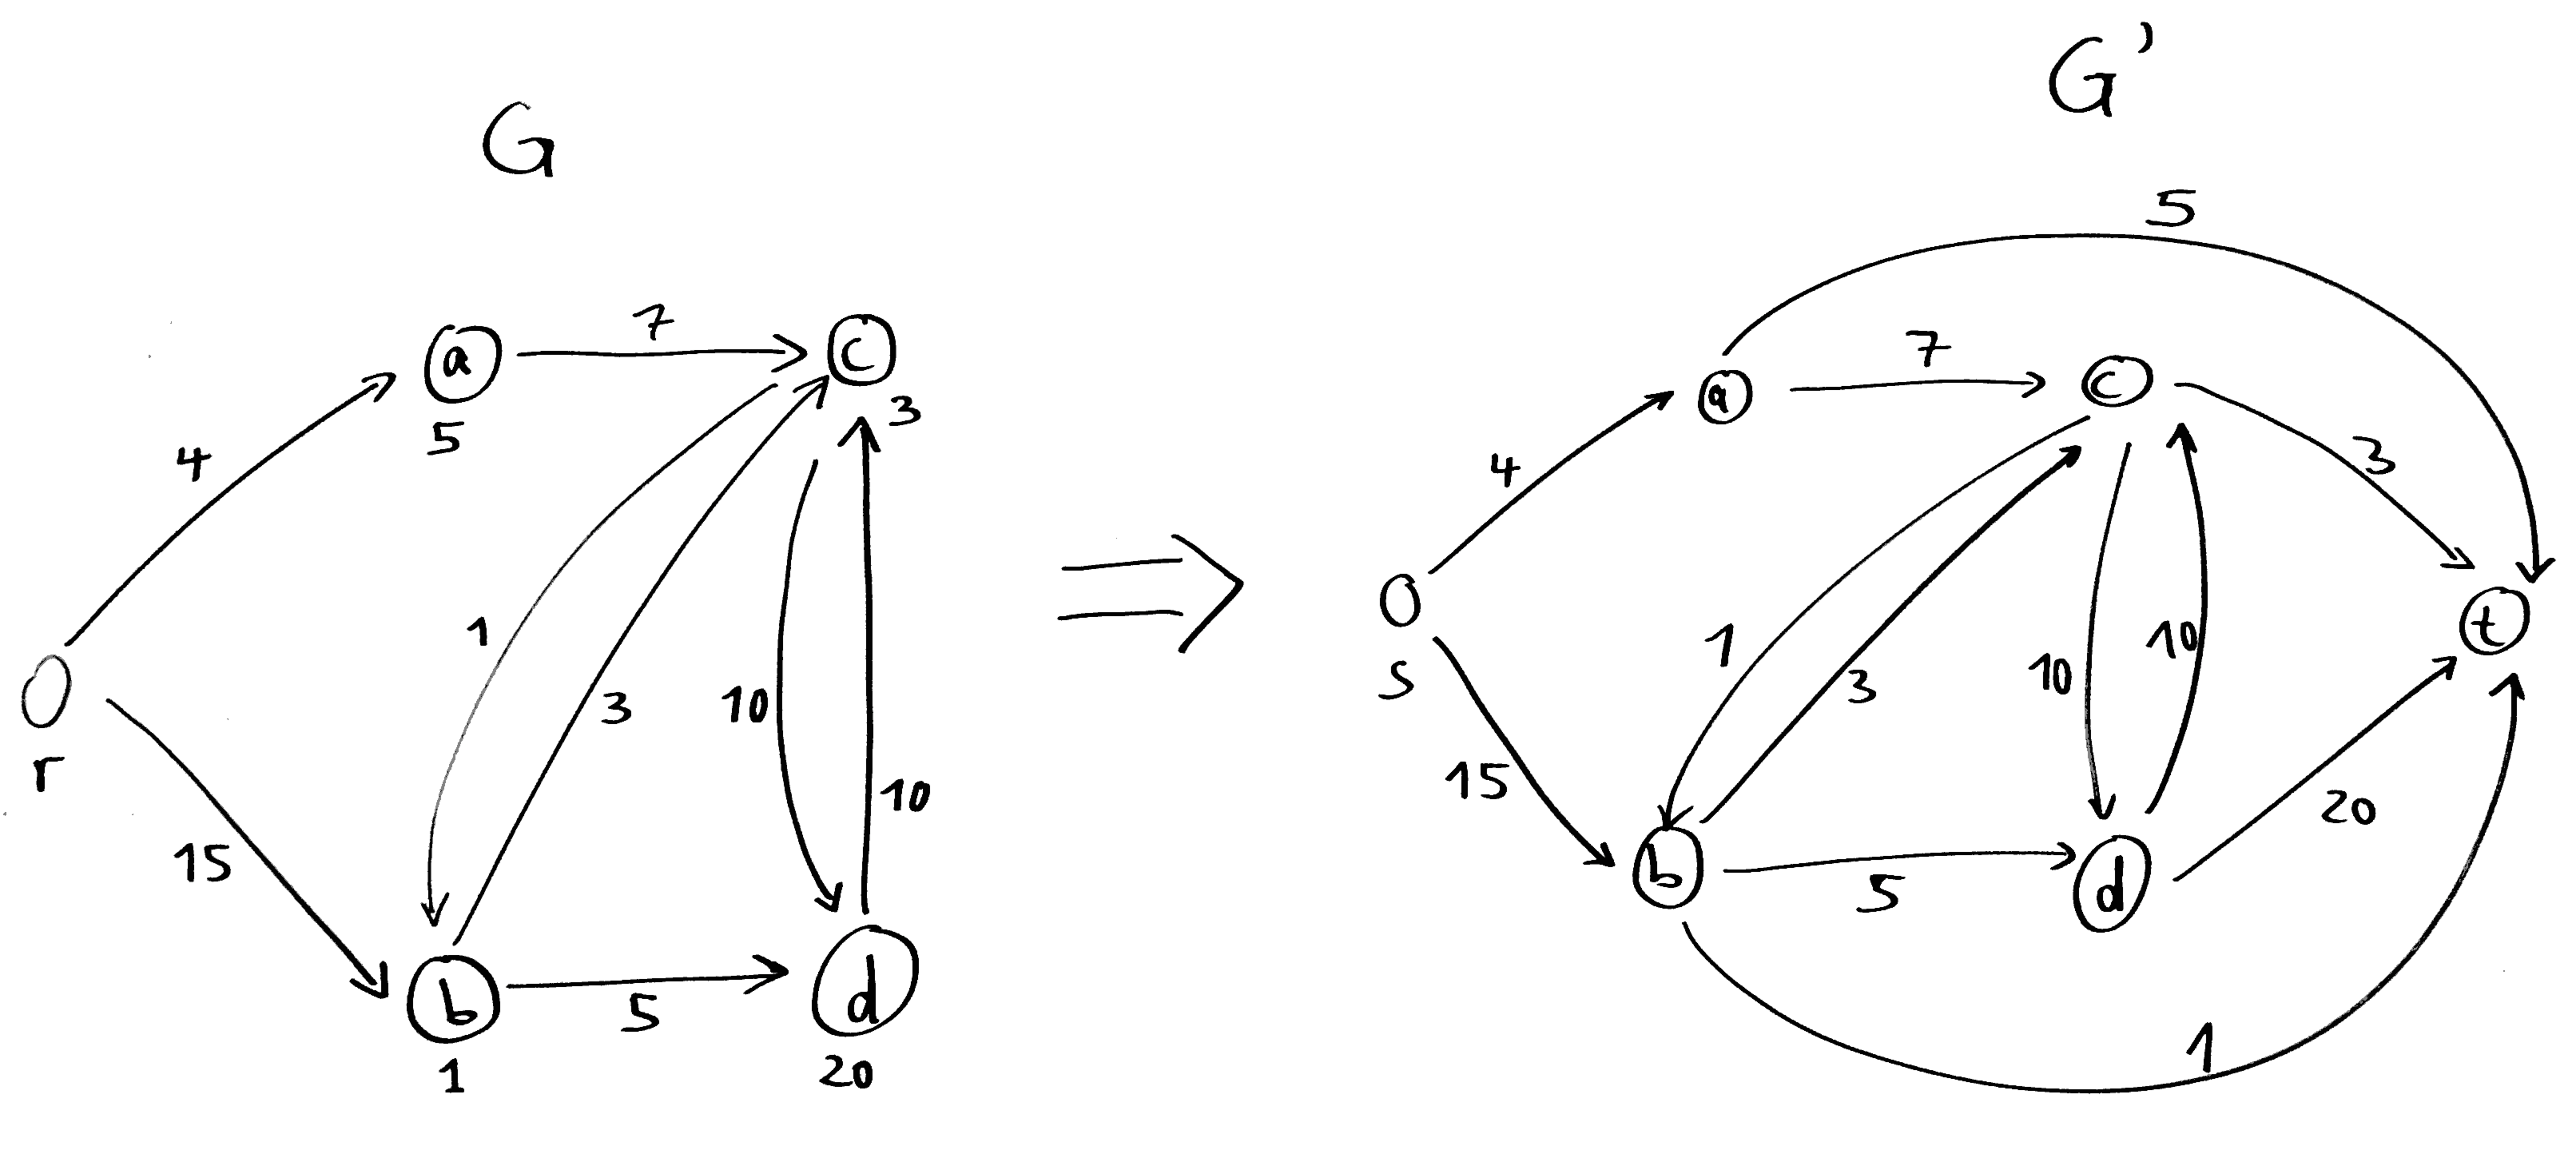
\includegraphics[width=\textwidth]{1_1.pdf}
\begin{itemize}
	\item Build a network flow graph $G'$ and calculate the minimum cut.
	\begin{itemize}
		\item Take the original graph.
		\item Connect every vertex $v \in V$ to the sink using a capacity of $b_v$. Adding such an edge to the cut means not to disconnect $v$ and not to get the benefit $v$.
	\end{itemize}
	\item Cut all edges that are in the minimal cut and part of the original graph.
\end{itemize}

\subsection*{Intuition}
\begin{itemize}
	\item We want to maximize the benefits of all disconnected vertices minus the cost for cutting the edges.
	\item Let $A,B$ a partitioning of $V$, such that $r \in V$.
	\item $\mbox{maximize } \sum_{b \in B} v_b - \mathit{cap}(A, B) \Leftrightarrow \mbox{minimize } \mathit{cap}(A, B) - \sum_{b \in B} v_b \Leftrightarrow \mbox{minimize } \mathit{cap}(A, B) + \sum_{a \in A} v_a$
	\item Restate the problem: minimize the costs for cutting edges plus the benefits that we do not get.
\end{itemize}

\subsection*{Network Flow Construction}
\begin{itemize}
	\item Start with the original graph $G=(V,E)$.
	\item Let the special vertex $r$ be the source $r=s$ and add an additional sink vertex $t$.
	\item For every vertex $v \in V - \{s, t\}$, add an edge $(v, t)$ called $e_v$ with capacity $v_b$.
	\item Call the new graph $G' = (V', E')$.
\end{itemize}

\subsection*{Full Algorithm}
\begin{algorithm}
  \caption{Partitioning/cutting $V$ in $A$ and $B$, such that $\sum_{b \in B} v_b - \mathit{capacity}(A,B)$ is maximized in $G$}
  \begin{algorithmic}[1]
    \Require{Graph $G=(V,E)$}
	%\Statex
    \Function{Max\-Benefit}{$G$}
		\State $G' \gets \mbox{build flow graph out of $G$}$
		\State $A,B \gets \mbox{calculate minimum cut in $G'$}$
		
		\State \Return $\mbox{all cut edges $e$ with $e \in E$}$
    \EndFunction
  \end{algorithmic}
\end{algorithm}

In this algorithm, we can calculate the minimum cut by running the Ford-Fulkerson algorithm or the Edmonds-Karp algorithm and determining which vertices are reachable from the source. These vertices form the set $A$. The cut edges are all edges $e=(u,v) \in E$ with $u \in A$ and $v \not \in  A$.

\subsection*{Proof}
We prove that the set of edges that are output by the algorithm, maximizes the profit if all these edges are removed.

\begin{itemize}
	\item \emph{Termination:} We assume that all $b_v$ and $c_e$ are rational numbers. Then, the Ford-Fulkerson algorithm is guaranteed to terminate.
	\item Reformulate the problem: We reformulate the original problem several times until we reach the min-cut formulation and show that the new formulation is equivalent to the previous one (if not trivial).
	\begin{itemize}
		\item \emph{Original problem:} Find a subset of edges $S \subseteq E$, such that $\sum_{b \in B} v_b - \sum_{e \in S} c_e$ is maximized, where $B$ is the set of vertices that is no longer reachable from $r$.
		\item Find $S \subseteq E$, such that $\sum_{e \in S} c_e - \sum_{b \in B} v_b$ is minimized.
		\item Find $S \subseteq E$, such that $\sum_{e \in S} c_e + \sum_{a \in V-B} v_a$ is minimized. $B$ and $V-B$ are complementary sets, i.e. maximizing $\sum_{b \in B} v_b$ is the same as minimizing $\sum_{a \in V-B} v_a$.
		\item Find a partitioning of $V$ in $B$ and $V-B=A$, such that $\sum_{e=(u,v) \in E: u \in A \wedge v \in B} c_e + \sum_{a \in A} v_a$ is minimized. $V-B=A$ is the set of vertices that is reachable from $r$. The choice of $A$ and $B$ determines the choice of edges $S$ (and vice-versa), i.e. the mapping from $A$/$B$ to $S$ is bijective. Given a set $S$ or $A$/$B$, we can also reconstruct the other set $A$/$B$ or $S$. Therefore, it does not matter whether we select $S$ or $A$/$B$.
		\item \emph{Model vertices as edges:} Generate flow network graph $G'$. Find the minimum cut. In the min-cut of $G'$, there must be no connection from $s$ to $t$. For every $v \in V$ in $G$, we either have to cut $e_v = (v,t)$ with capacity $b_v$ in $G'$ or cut edges, such that $v \in B$. If $v \in A$, we have to pay the cost for cutting $e_v$. Therefore, this problem is equivalent to the previous one.
	\end{itemize}
\end{itemize}

\subsection*{Runtime Complexity}
\begin{itemize}
	\item Building the flow network: we generate $\mathcal{O}(|V|)$ vertices and $\mathcal{O}(|E| + |V|)$ edges, where $|V|$ is the number of vertices in $G$ and $|E|$ is the number of edges in $G$.
	\item Calculating the max-flow with the Edmonds-Karp algorithm: $\mathcal{O}(|V'| |E'|^2)=\mathcal{O}(|V'|^5)$ (worst case: fully connected graph, i.e. $|E'| = \mathcal{O}(|V'|^2)$. In terms of $G$, calculating the max-flow takes $\mathcal{O}(|V|^5)$ time.
	\item Retrieving the min-cut/partitioning: run DFS from $r$ in $\mathcal{O}(|V'| + |E'|) = \mathcal{O}(2|V| + |E|) = \mathcal{O}(|V| + |E|)$.
	\item Overall runtime complexity: $\mathcal{O}(|V|^5)$.
\end{itemize}

\newpage
\section*{Problem 4: Approximating the independent set}
\subsection*{LP relaxation}
\begin{itemize}
	\item $\mbox{Maximize } \sum_{v \in V} x_v$
	\item subject to
	\begin{itemize}
		\item $\forall e=(u,v) \in E: x_u + x_v \leq 1$
		\item $\forall v \in V: x_v \geq 0$
	\end{itemize}
\end{itemize}

\subsection*{Polynomial time algorithm}
In this section, we give a polynomial time algorithm that either finds an independent set of at least $\frac{|V|}{3}$ in $G$ or certifies that no independent set of size greater or equal to $\frac{2 |V|}{3}$ exists.

\subsubsection*{Basic Idea}
\begin{itemize}
	\item We describe a 2-approximation algorithm of the minimal vertex cover problem using linear programming and constraint the vertex cover to be at most of size $\frac{|V|}{3}$ in the relaxed problem.
	\item If the LP is feasible, we round the values. We will end up with a vertex cover of size $\leq \frac{2 |V|}{3}$, resulting in an independent set of size $\geq \frac{|V|}{3}$.
	\item If the LP is infeasible, we can show that no independent set of size $\geq \frac{2 |V|}{3}$ exists.
\end{itemize}

\subsubsection*{LP relaxation and 2-approximation for Vertex Cover}
The minimal vertex cover problem can be written as a relaxed linear program as follows.
\begin{itemize}
	\item $\mathit{Minimize } \sum_{v \in V} x_v$
	\item subject to
	\begin{itemize}
		\item $\forall e=(u,v) \in E: x_u + x_v \geq 1$
		\item $\forall v \in V: x_v \geq 0$
	\end{itemize}
\end{itemize}

We can approximate the minimal vertex cover with a factor of $2$ as follows.
\begin{itemize}
	\item For every $v \in V$, set $x_v$ to $1$ if $x_v \geq 0.5$ (round up) and set $x_v$ to $0$ if $x_v < 0.5$ (round down).
	\item $T_{\mbox{LP}} = \{v \left.\right| v \in V: x_v = 1\}$ is a vertex cover, because, for every edge $e = (u,v) \in E$, at least one of value of $x_u$ and $x_v$ will be $1$. Because of the first constraint in the linear program, $x_vu$ and $x_v$ can never be both smaller than $0.5$ in the relaxed version. Therefore, at least one of them is rounded to $1$ and, therefore, every edge is covered.
	\item $T_{\mbox{LP}}$ is a 2-approximation. The objective function value of the relaxed LP is a lower bound for the size of the minimal vertex cover\footnote{If there was a smaller vertex cover, then the linear program would have found it (or an even smaller solution with fractions).}. In the worst case, all $x_v =0.5$ in the relaxed version. Therefore, we round all $x_v$ to $1$, resulting in an upper bound of $|V|$ for the approximation. Therefore, the approximation factor is $\frac{|V|}{0.5 |V|} = 2$.
\end{itemize}

\subsubsection*{Duality of Vertex Cover and Independent Set\footnote{Proof taken from Kleinberg, Tardos textbook, page 455.}}
Let $G=(V,E)$ be a graph. Then $S$ is an independent set if and only if $V-S$ is a vertex cover. Let $e=(u,v) \in E$ be an arbitrary edge. $u$ and $v$ cannot be part of $S$ at the same time, so $V-S$ is a vertex cover. Assume that $V-S$ is a vertex cover and let $e=(u,v) \in E$ be an arbitrary edge with $u \in S$ and $v \in S$. Then, neither $v \in V-S$, nor $u \in V-S$, contradicting our assumption that $V-S$ is a vertex cover. Therefore, $u$ and $v$ cannot be part of $S$ at the same time and $S$ is an independent set.

\subsubsection*{Full Algorithm}
\begin{algorithm}
  \caption{Finding an independent set of size at least $\frac{|V|}{3}$ or stating that no independent set of size at least $\frac{2 |V|}{3}$ exists.}
  \begin{algorithmic}[1]
    \Require{Graph $G=(V,E)$}
	%\Statex
    \Function{One\-Third\-Independent\-Set}{$G$}
		\State $P \gets \mbox{relaxed LP for the minimal vertex cover for $G$}$
		\State $\mbox{Add constraint $\sum_{v \in V} x_v \leq \frac{|V|}{3}$ to $P$}$
		\State $\mbox{Solve $P$ with the Ellipsoid method}$
		\If{$\mbox{$P$ is infeasible}$}
			\State \Return $\mbox{No independent set of size $> \frac{2 |V|}{3}$}$
		\Else
			\State \Return $\{v \left.\right| v \in V: x_v < 0.5 \mbox{ in $P$}\}$
		\EndIf
    \EndFunction
  \end{algorithmic}
\end{algorithm}

\subsubsection*{Proof}
\begin{itemize}
	\item Let $P$ be the relaxed LP of the minimum vertex cover problem with the constraint that the vertex cover must be at most of size $\frac{|V|}{3}$. Let $x_v$ be the decision variable values in its solution.
	\item Case 1: $P$ is feasible.
	\begin{itemize}
		\item Let $\tilde{x}_v$ be the rounded values of $x_v$. Let $C = \{v \in V \left.\right| \tilde{x}_v = 1\}$.
		\item $C$ is a 2-approximation of the minimal vertex cover in $G$\footnote{Proof: see approximation section.}.
		\item $\sum_{v \in V} x_v \leq \frac{|V|}{3} \Rightarrow \sum_{v \in V} \tilde{x}_v = |C| \leq \frac{2 |V|}{3}$
		\item Let $S = V - C$. $S$ is an independent set and $|S| \geq |V| - \frac{2 |V|}{3} = \frac{|V|}{3}$.
	\end{itemize}
	\item Case 2: $P$ is infeasible.
	\begin{itemize}
		\item $G$ has no vertex cover of size $\leq \frac{|V|}{3}$. Otherwise, the LP would have found an assignment of $x_i$ with such an objective function value. 
		\item Let $C$ be the minimum vertex cover in $G$ and $S$ be the maximum independent set in $G$.
		\item $|C| > \frac{|V|}{3} \Rightarrow |S| \leq |V| - |C| = \frac{2 |V|}{3}$.
		\item There is no independent set of size $> \frac{2 |V|}{3}$. \hfill $\blacksquare$
	\end{itemize}
\end{itemize}

\subsubsection*{Runtime Complexity}
\begin{itemize}
	\item Building the linear program: we create $|V|$ variables, add $|V|$ non-negativity constraints and $|E|$ edge constraints. Therefore, the size of the linear program is polynomial in the size of $G$.
	\item The Ellipsoid method solves the linear program in polynomial time.
	\item The overall runtime complexity of the algorithm is polynomial in the size of $G$.
\end{itemize}

\subsection*{Polynomial time algorithm for graphs of degree 3}
\subsubsection*{Basic Idea}
\begin{itemize}
	\item The idea from the previous subproblem can be generalized: given an $\phi$-approximation algorithm of the vertex cover, we can came up with an algorithm that
	\begin{itemize}
		\item finds an independent set of size at least $\alpha |V| = \frac{|V|}{1 + \phi}$ or
		\item or certifies that no independent set has size greater than $(1 - \alpha) |V| = \frac{\phi |V|}{1 + \phi}$
	\end{itemize}
	\item The quality of the vertex cover approximation determines the value $\alpha$.
\end{itemize}

\subsubsection*{Full Algorithm}
The following algorithm is a general algorithm that works with any $\phi$-approximation of the minimum vertex cover problem and yields an $\alpha = \frac{1}{1 + \phi}$.
\begin{algorithm}
  \caption{Finding an independent set of size at least $\alpha |V|$ or stating that no independent set of size at least $(1-\alpha) |V|$ exists.}
  \begin{algorithmic}[1]
    \Require{Graph $G=(V,E)$}
	%\Statex
    \Function{$\alpha$\-Independent\-Set}{$G$}
		\State $\beta \gets 1 - \alpha$
		\State $S \gets \mbox{$\phi$-approximation for minimum vertex cover}(G)$
 
		\If{$|S| > \beta$}
			\State \Return $\mbox{No independent set of size $> (1-\alpha) |V|$}$
		\Else
			\State \Return $V-S$
		\EndIf
    \EndFunction
  \end{algorithmic}
\end{algorithm}

\subsubsection*{Proof}
\begin{itemize}
	\item The run of the $\phi$-approximation algorithm for the minimum vertex cover on $G$ can have two possible outcomes. Let $S$ be the $\phi$-approximated minimum vertex cover.
	\item Case 1: $|S| \leq \beta |V|$
	\begin{itemize}
		\item The approximated minimum vertex cover has size $|S| \leq \beta |V|$.
		\item There is an independent set of size $\geq (1-\beta) |V|$.
	\end{itemize}
	\item Case 2: $|S| > \beta |V|$
	\begin{itemize}
		\item The approximated minimum vertex cover has size $> \beta |V|$. Therefore, the real minimum vertex cover has size $> \frac{1}{\phi} \beta |V|$
		\item The maximum independent set has size $< (1 - \frac{\beta}{\phi}) |V|$. Therefore, there is no independent set of size $\geq (1 - \frac{\beta}{\phi}) |V|$.
	\end{itemize}
	\item We must set $\beta = (1 - \frac{\beta}{\phi}$\footnote{This is equivalent to $1-\beta = \frac{\beta}{\phi}$.}, otherwise, we end up with an interval between these two terms, where we cannot say whether the independent set exists or not. For a given $\phi$, $\beta = (1+\phi^{-1})^{-1} = \frac{\phi}{\phi+1}$.
	\item For $\alpha = 1-\beta$, we get relations in terms of the independent set that match the previously mentioned formulas in the \emph{Basic Idea} section.
	\begin{itemize}
		\item Find an independent set of size at least $\alpha |V| = (1-\beta) |V| = (1-\frac{\phi}{\phi + 1}) |V| = \frac{|V|}{\phi + 1}$ or
		\item certifies that no independent set of has size greater than $(1-\alpha) |V| = \beta |V| = \frac{\phi}{\phi + 1} |V|$
	\end{itemize}
	\item The quality of the the approximation determines the value of $\alpha$ that we get. For example, for the 2-approximation in the previous subproblem, we get $\alpha = \frac{1}{\phi + 1} = \frac{1}{3}$. By finding a better approximation of the minimum vertex cover, we can increase $\alpha$. \hfill $\blacksquare$
\end{itemize}

\subsubsection*{$\frac{3}{2}$-approximation for Vertex Cover}
\begin{itemize}
	\item Given an $\phi$-approximation algorithm, we can immediately calculate a value of $\alpha$ and give an algorithm that finds an independent set of size $\alpha |V|$ or certifies that no independent set has size greater than $(1-\alpha) |V|$, according to the previous argument.
	\item Algorithm: select the vertex with the highest degree, add it to the vertex cover, and remove it.
	\item For graphs with a maximum degree of 3, this is a $\frac{3}{2}$-approximation.
	\item In the worst case, the graph consists of cliques of size $4$, i.e. every vertex in every clique has $3$ connections. In that case, the minimum vertex cover is $\frac{3 |V|}{4}$, because only $3$ vertices cover all $6$ edges per clique.
	\item The minimum number of vertices that a vertex cover must cover is $\frac{|V|}{4}$. Consider the case, where the graph consists of disconnected components of $4$ vertices, where one vertex is in the middle and the other $3$ vertices are connected to only this middle vertex. \textsc{Insert more Proof here}.
	\item Therefore, according to the previous argumentation and proof, we get an algorithm with $\alpha=\frac{1}{1+\frac{3}{2}} = \frac{2}{5}$.
\end{itemize}

\newpage
\section*{Problem 5: Always non-negative path}
\subsection*{Basic Idea}
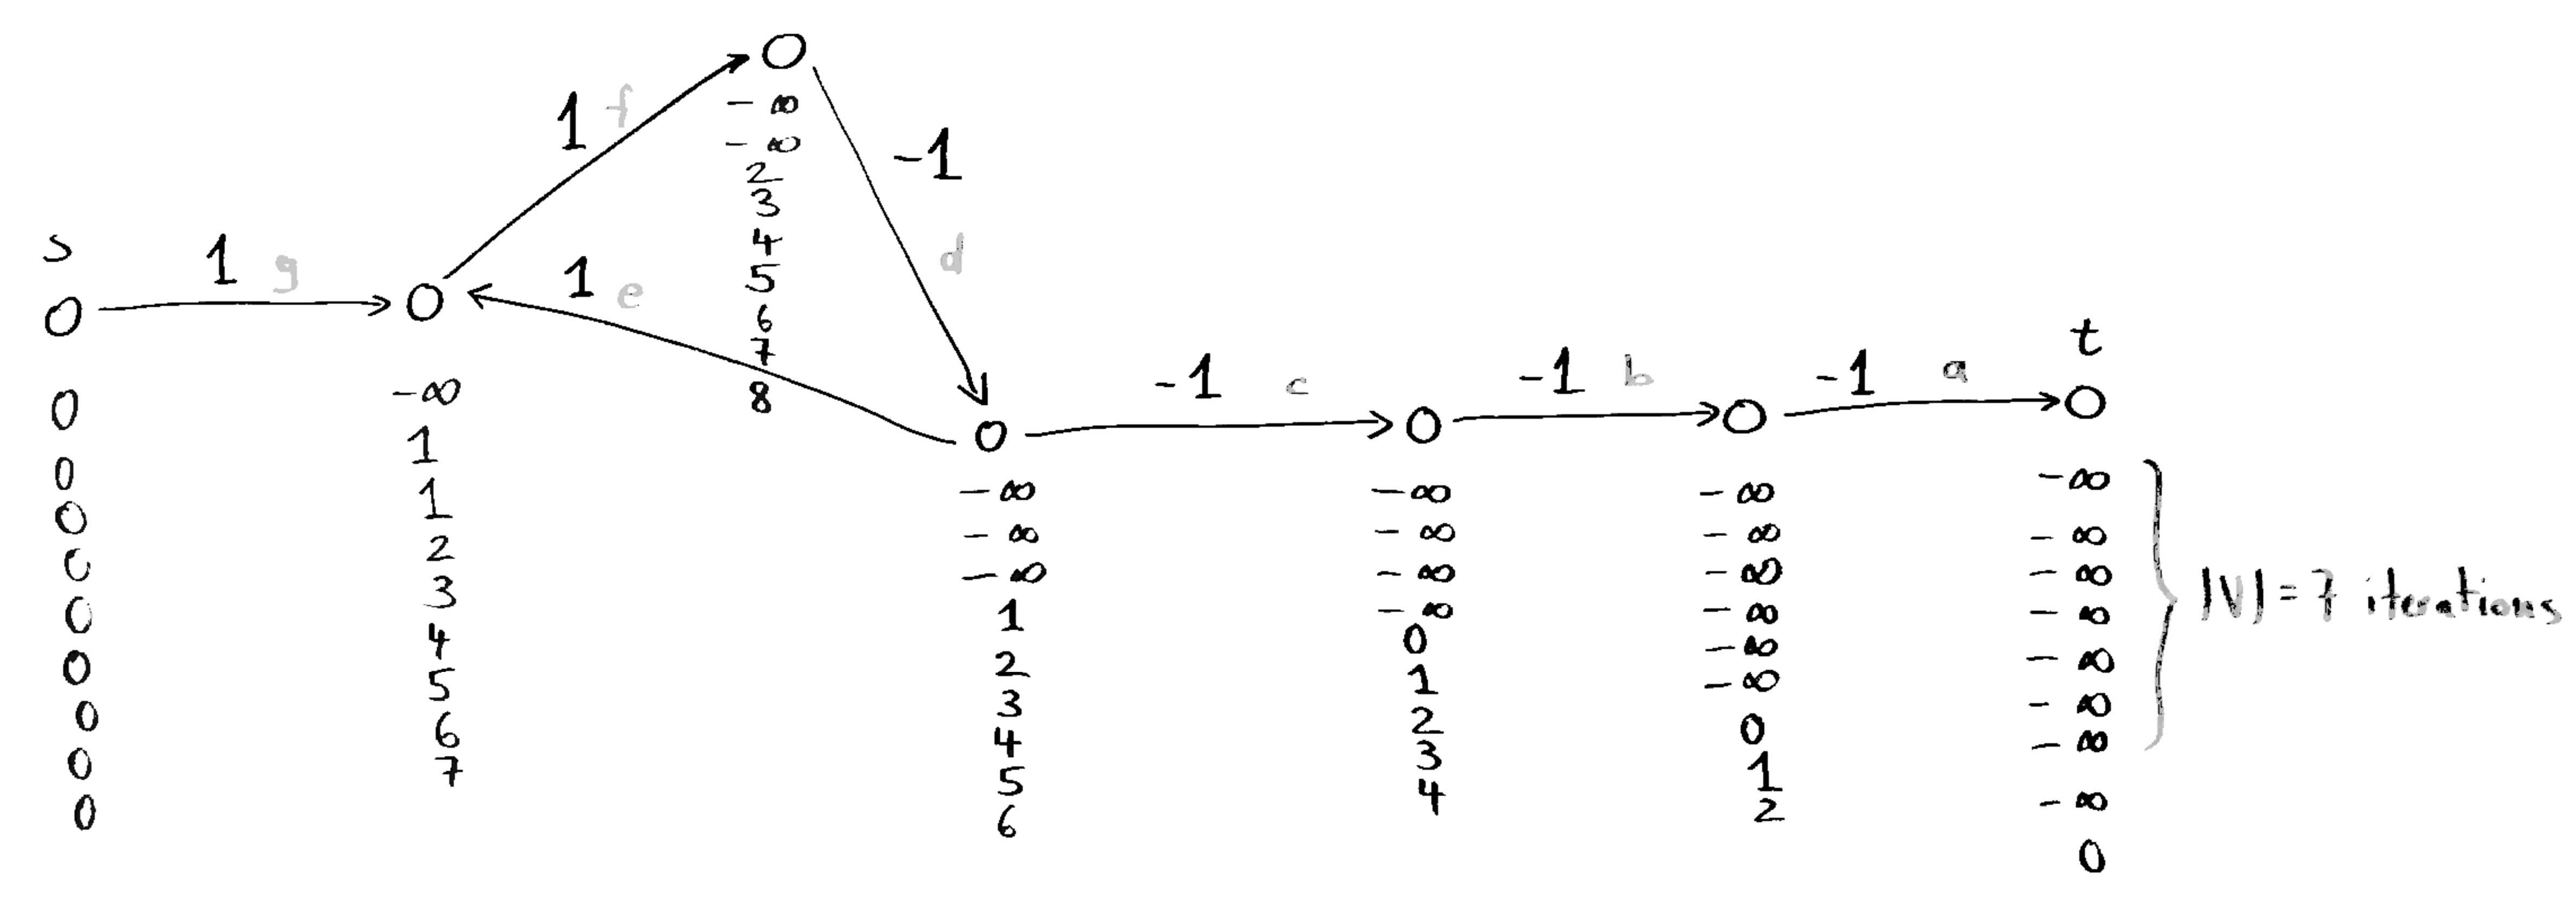
\includegraphics[width=\textwidth]{5_1.pdf}
\begin{itemize}
	\item The algorithm is similar to the Bellman-Ford algorithm. Iterate over all edges $e=(u,v) \in E$, $|V|$ times, and update $\mathit{maxSum}[v]$, i.e. the maximum achievable sum on an always non-negative $s$-$v$ path.
	\item $\forall e=(u,v) \in E$: $\mathit{maxSum}[v] \gets \max \{\mathit{maxSum}[v], \mathit{maxSum}[u] + w(e) \mbox{ \textbf{if} } \mathit{maxSum}[u] + w(e) \geq 0\}$, where $w(e)$ is the weight of edge $e$. Repeat this step $|V|$ times (\emph{Bellman-Ford} step).
	\item As we can see in the illustration above, we might have to cycle in positive-weight cycles multiple times, in order to accumulate a value that is big enough to make up for a long sequence of $-1$ edges on the rest of the $s$-$t$ path.
	\item We find the first reachable strictly-positive-weighted cycle, i.e. a positive-weight cycle $C$ with $\forall v_C \in C: \mathit{maxSum}[v_C] \geq 0$, on an $s$-$t$ path using DFS (if there is such a cycle) and set all $\mathit{maxSum}[v_C] = \infty$\footnote{It is crucial that all $\mathit{maxSum}$ values are $\geq 0$, because we would not be allowed to use the cycle in the first place if it cannot be reached by any always non-negative path.}.
	\item We repeat the Bellman-Ford step, updating the $\mathit{maxSum}$ values and using strictly-positive-weighted loops arbitrarily often if necessary.
	\item There is an always non-negative $s$-$t$ path if and only if $\mathit{maxSum}[t] \geq 0$.
\end{itemize}

\subsection*{Full Algorithm}
\begin{itemize}
	\item The Bellman-Ford step is very similar to the the Bellman-Ford algorithm. Instead of trying to reduce the path length, we try to find a path weight that is as big as possible. We only use vertices with a non-negative path length, ensuring that this condition holds for subpaths starting from $s$.
	\item The DFS step runs a depth-first search using a stack. We somehow need to store, whether a vertex was already visited, e.g. by using an array. Once we reach an already visited vertex $v$, we compare the sum that we accumulated so far with $\mathit{maxSum}[v]$. If the accumulated sum is greater, then we found a strictly-positive-weighted cycle and increase all vertices on that cycle\footnote{The cycle vertices are all vertices on the stack up to the vertex $v$, i.e. all vertices on the stack between $v$ and the current vertex (including these vertices).} to infinity. We do not visit vertices $u$ with a negative value of $\mathit{maxSum}[u]$, ensuring that we only visit vertices that can be reached by an always non-negative path.
\end{itemize}

\begin{algorithm}
  \caption{Deciding whether there is an always non-negative $s$-$t$ path in $G$.}
  \begin{algorithmic}[1]
    \Require{Graph $G=(V,E)$}

    \Function{Always\-Non\-Negative}{$G$}
		\State $\forall v \in V: \mathit{maxSum}[v] \gets -\infty$
		\State $\mathit{maxSum}[s] \gets 0$
		\State \Call{Bellman\-Ford\-Step}{\null}
		\State \Call{Dfs\-Step}{\null}
		\State \Call{Bellman\-Ford\-Step}{\null}
		\State \Return $\mathit{maxSum}[t] \geq 0$
    \EndFunction
  \end{algorithmic}
\end{algorithm}

\begin{algorithm}
  \caption{Adapting $\mathit{maxSum}$ for all $v \in V$ by propagating all these values using every edge $|V|$ times.}
  \begin{algorithmic}[1]
    %\Require{Graph $G=(V,E)$}

    \Function{Bellman\-Ford\-Step}{\null}
		\For{$i \gets 1 \mbox{ \textbf{to} } |V|$}
			\ForAll{$e = (u,v) \in E$}
				\If{$\mathit{maxSum}[u] + w(e)\geq 0$}
					\State $\mathit{maxSum}[v] \gets \max \{\mathit{maxSum}[v], \mathit{maxSum}[u] + w(e)\}$
				\EndIf
			\EndFor
		\EndFor
    \EndFunction
  \end{algorithmic}
\end{algorithm}

\begin{algorithm}
  \caption{Setting $\mathit{maxSum}[v] \gets \infty$ for all $v \in C$ for at least the first reachable strictly-positive-weighted cycle $C$ on every always non-negative $s$-$t$ path.}
  \begin{algorithmic}[1]
    %\Require{Start vertex $x$}

    \Function{Dfs\-Step}{\null}
		\State $S \gets \mbox{ new Stack}$
		\State $\mathit{maxSum}_\mathit{old} \gets \mbox{copy}(\mathit{maxSum})$
		\State $S.\mbox{push}((s, 0))$
		\While{$|S| > 0$}
			\State $(v, m) \gets S.\mbox{peek}()$
			\State $\mbox{mark $v$ as visited}$
			\ForAll{$u \in V: (v,u) \in E$}
				\If{$\mathit{maxSum}_\mathit{old} \geq 0$}
					\If{$u \mbox{ was already visited}$}
						\If{$u \in S \wedge m + w(e_{v,u}) > \mathit{maxSum}_\mathit{old}[u]$}
							\ForAll{$a \in V: (a, x) \in S \wedge \mbox{ $(a,x)$ is not before $(u,y)$ in $S$}$}
							% we found a cycle and the weight increased
								\State $\mathit{maxSum}[a] \gets \infty$
							\EndFor
						\Else
							\State $S.\mbox{push}(u, m + w(e_{v,u}))$
						\EndIf
					\EndIf
				\EndIf
			\EndFor
			\State $S.\mbox{pop}()$
		\EndWhile
    \EndFunction
  \end{algorithmic}
\end{algorithm}

\subsection*{Proof}

\begin{frm-thm}
After the first \textsc{BellmanFordStep}, for all $v \in V$, $\mathit{maxSum}[v]$ is the maximum sum of all always non-negative $s$-$v$ paths of length $\leq |V|$, if such a path exists, and $-\infty$ otherwise.
\end{frm-thm}

We prove this by induction over the number of used edges $k$, that after $k$ iterations of the outer loop, $\mathit{maxSum}[v]$ is the maximum sum of all always non-negative $s$-$v$ paths using at most $k$ edges.

\begin{itemize}
	\item \emph{Induction Base Case:} For $k=0$, we are not allowed to use any edge. Therefore, $\mathit{maxSum}[s] = 0$ and for all other vertices $v \in V - \{s\}$, $\mathit{maxSum}[v] = -\infty$.
	\item \emph{Induction Hypothesis:} Let the statement be true for an arbitrary but fixed $k$.
	\item \emph{Induction Step:} When we update $\mathit{maxSum}[v]$, for some $v \in V$ and $e=(u,v) \in E$, we set $\mathit{maxSum} = \mathit{maxSum} + w(e)$. We only do this if the new value of $\mathit{maxSum}[v]$ is non-negative. $\mathit{maxSum}[u] \geq 0$, because we never set $\mathit{maxSum}$ to a negative value (except for the initialization), and, by induction, $\mathit{maxSum}[u]$ is the maximum sum of all always non-negative $s$-$u$ paths using $k-1$ edges. In every iteration, we try to improve paths using all possible edges, and only update $\mathit{maxSum}$ if it becomes greater. Therefore, at the end of $k$th iteration, $\mathit{maxSum}[v]$ is the maximum sum of all always non-negative $s$-$v$ paths using at most $k$ edges. If $\mathit{maxSum}[v] = -\infty$, it was not updated because $v$ is not reachable from $s$ using an always non-negative path with at most $k$ edges.
\end{itemize}

\begin{frm-thm}
Let $P$ be an arbitrary $s$-$t$ path, and $C$ be a strictly-positive-weighted cycle $C$ with $P \cap C \not= \emptyset$, such that $C$ is the first such cycle for $P$ and for all $v_c \in C$, there exists an always non-negative $s$-$v_c$ path in $G$. After \textsc{DfsStep}, for all $v_c \in C$, $\mathit{maxSum}[v_c] = \infty$.
\end{frm-thm}

When the DFS visits a vertex, it accumulates the edge sum for the current path starting from $s$. When it reaches an already visited vertex $v$ and $v$ is not on the stack anymore, then we found an undirected, but no directed cycle. If $v$ is still on the stack, then all vertices starting from $v$ to the top of the stack form a cycle $C$\footnote{If there was a vertex $u \in V$ among these vertices, that is not part of the cycle, then the DFS would not have been able to continue the path to $v$ and popped $u$ from the stack.}. The algorithm takes all these vertices and sets their $\mathit{maxSum}$ values to $\infty$.

Let us assume that a vertex $v_c \in C$ is not reachable by an always non-negative $s$-$v_c$ path in $G$. Then, at least one vertex $u$ on any $s$-$v_c$ path has $\mathit{maxSum}[u] = -\infty$. Then, the DFS will not visit this vertex and there is no way to find the cycle, because, either a vertex on the path to the cycle is not visited, or a vertex inside the cycle is not visited.

Note, that this works only, because $\mathit{maxSum}[v]$ contains the maximum sum of all always non-negative $s$-$v$ paths using at most $|V|$ edges. Since $C$ is the first cycle on an $s$-$t$ path, there is no way to accumulate a high edge sum in order to reach $C$ with an always non-negative path. Therefore, if a cycle $|C|$ cannot be reached by an always non-negative path using at most $|V|$ edges (which can involve all vertices), then $C$ cannot be reached by an always non-negative path at all.

\begin{frm-thm}
There is an always non-negative $s$-$t$ path in $G$, if and only if
\begin{itemize}
	\item $t$ can be reached from $s$ via an always non-negative path of length at most $|V|$ or
	\item there is an always non-negative path of length at most $|V|$ to a strictly-positive-weighted cycle $C$, and some $v_C \in C$ has an arbitrary path to $t$.
\end{itemize}
\end{frm-thm}

In the first case, the algorithm finds that path in the first \textsc{BellmanFordStep} according to the first lemma. In the second case, the algorithm find the first strictly-positive-weighted cycle $C$ that insects with $P$, where $P$ is some always non-negative $s$-$t$ path. The distance $C$ from $s$ cannot be greater than $|V|$, because, otherwise, we would have to visit a vertex twice, which results in a cycle, contradicting our assumption that $C$ is the first such cycle. After we reached the cycle $C$, we can loop in it as often as we want to and accumulate an arbitrary high $\mathit{maxSum}$ value, therefore $\mathit{maxSum}[v_C] = \infty$. Therefore, $t$ is reachable using an always non-negative path from $v_C$, regardless of the weights on that path. Using the same argument from the first lemma, we can prove that by running \textsc{BellmanFordStep} again, we update all $\mathit{maxSum}[u] = \infty$ for every vertex $u$ on any $v_C$-$t$ path. Therefore, the algorithm sets $\mathit{maxPath}[t] = \infty$ and outputs the correct answer. 

If none of the two cases applies, then there is no simple always non-negative $s$-$t$ path and there is no way to increase the sum in loop that leads to $t$. Therefore, $\mathit{maxSum}[t] = -\infty$ after the first \textsc{BellmanFordStep} (according to the first lemma), and either \textsc{DfsStep} does not change $\mathit{maxSum}$ values or there is no way from the loop to $t$, in which case the second \textsc{BellmanFordStep} cannot propagate the increased values to $t$. \hfill $\blacksquare$

\subsection*{Runtime Complexity}
\begin{itemize}
	\item Running \textsc{BellmanFordStep}: $|V|$ iterations for the outer loop and $|E|$ iterations for every inner loop run, resulting in $\mathcal{O}(|V| |E|)$ iterations.
	\item Running \textsc{DfsStep}: The runtime of DFS is $\mathcal{O}(|V| + |E|)$. In the worst case, we update no more than $|V|$ $\mathit{maxSum}$ values per vertex, resulting in $\mathcal{O}(|V|^2 + (|V| + |E|)$.
	\item Running \textsc{BellmanFordStep} again: $\mathcal{O}(|V| |E|)$.
	\item The overall runtime complexity is $\mathcal{O}(|V| |E| + |V|^2 + |V| + |E| + |V| |E|)$. In the worst case, $|E| = |V|^2$ (fully connected graph), so the runtime complexity is $\mathcal{O}(|V|^3)$.
\end{itemize}
 
\newpage
\section*{Problem 2: Coupon Collector}
\subsection*{Basic Idea}
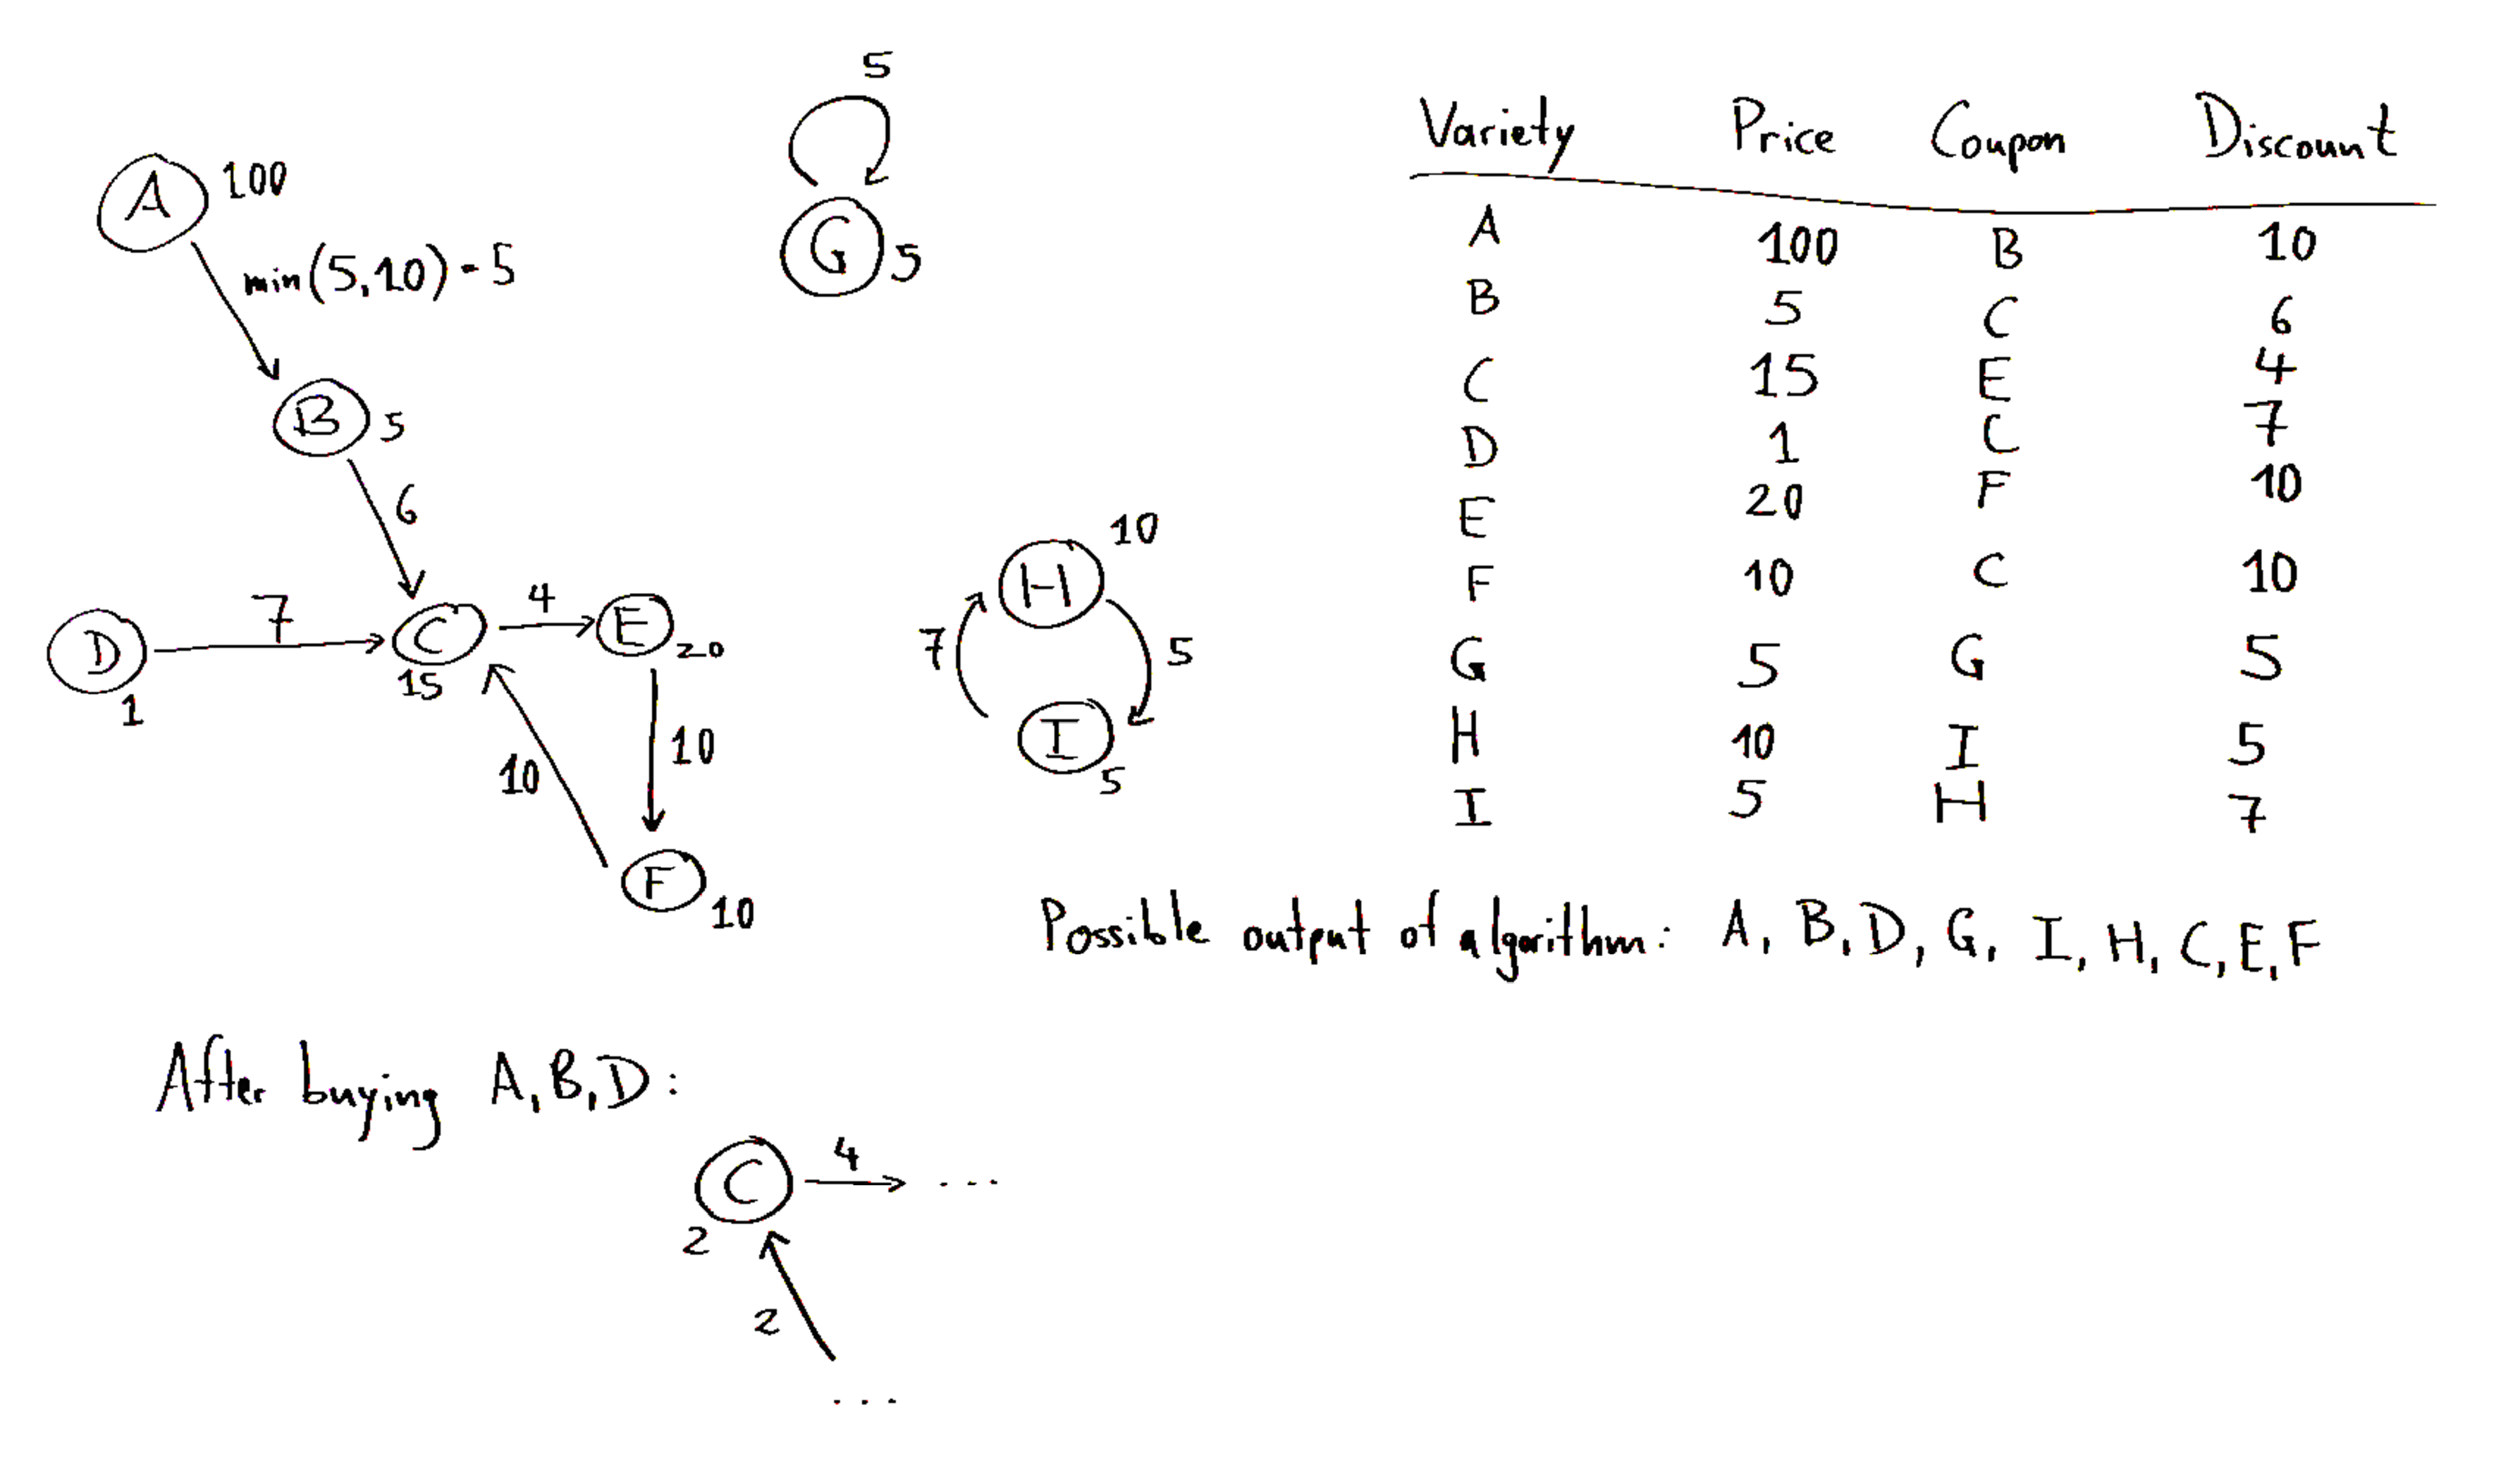
\includegraphics[width=\textwidth]{2_1.pdf}
\begin{itemize}
	\item Model the problem as a graph. Every variety $i$ gets a vertex $w_i = v_i$ with weight $p_i$. Add an edge $(v_i, v_j)$ with weight $w_{i,j} = \min \{p_j, v_i\}$, indicating that we might get a discount of $w_{i,j}$ if buy variety $i$ before variety $j$.
	\item \emph{Intuition:} Always buy the variety such that we will loose the smallest discount. After buying variety $i$ with a coupon for $j$, subtract $w_{i,j}$ from $w_j$, indicating that $j$ is now cheaper to buy. Update $j$'s incoming edges, such that their weight is not bigger than $w_j$ (you cannot save more money than the variety costs)\footnote{It is sufficient to update all edges at once only a single time after buying all varieties with no incoming edges, leading to linear runtime.}.
	\item Buy all varieties with no incoming edges first (we will loose no discount and we have to buy them anyway), until there are only cycles left (see proof).
	\item For every cycle $C$, buy the variety $i$ with $v_i \in C$, where $w_{j, i}$ is minimal and $(v_j, v_i) \in E$ (at this time, there can only be one incoming edge for every vertex), i.e. buy the variety where we loose the least discount. Buy the rest of the varieties in $C$ by following the edges in the cycle.
\end{itemize}

\subsection*{Graph Construction}
\begin{itemize}
	\item For every variety $i$, add a vertex $v_i$ with a weight $w_i = v_i$.
	\item If variety $i$ contains a coupon for variety $j$ with discount $v_i$ and the regular price of $j$ is $p_j$, add an edge $(v_i, v_j)$ with weight $w_{i,j} = \min \{p_j, v_i\}$.
\end{itemize}

\subsection*{Full Algorithm}
\begin{algorithm}
  \caption{Coupon Collector Algorithm}
  \begin{algorithmic}[1]
    %\Require{Graph $G=(V,E)$}

    \Function{Coupon\-Collector}{\null}
		\State $\mbox{build graph $G$}$
		\ForAll{$v \in V$}
			\If{$v \mbox{ was not yet visited}$}
				\State $\Call{DfsBuy}{v}$
			\EndIf
		\EndFor
		
		\State $\forall e=(u,v) \in E: w_{u,v} \gets \min \{w_{u,v}, w_{v} \}$
				
		\ForAll{$v \in V$}
			\State $s \gets \mbox{vertex $u$ in $v$'s cycle such that $w_{x,u}$ is minimal for some $x$}$
			\While{$s.\mbox{next} \not= \mbox{null}$}
				\State $\Call{buy}{s}$
				\State $s \gets s.\mbox{next}$
				\State $\mbox{delete}(s)$
			\EndWhile
		\EndFor
    \EndFunction
  \end{algorithmic}
\end{algorithm}

\begin{algorithm}
  \caption{Buy a variety and update the prices and achievable discounts}
  \begin{algorithmic}[1]
    \Require{Vertex $v$}

    \Function{DfsBuy}{v}
		\State $\mbox{mark $v$ as visited}$
		\If{$\mathit{deg}_\mathit{in}(v) = 0$}
			\State $\Call{buy}{v}$
			\State $\mbox{delete}(v)$
		\EndIf
		
		\If{$v.\mbox{next} \mbox{ was not yet visited}$}
			\State $\Call{DfsBuy}{v.\mbox{next}}$
		\EndIf
    \EndFunction
  \end{algorithmic}
\end{algorithm}

\begin{algorithm}
  \caption{Buy varieties with no other incoming edges}
  \begin{algorithmic}[1]
    \Require{Vertex $v$}

    \Function{Buy}{v}
		\State $w_{v.\mathit{next}} \gets w_{v.\mathit{next}} - w_{v, v.\mathit{next}}$
		\State $\mbox{buy variety}(v)$
		\State $\mbox{delete}(v)$

    \EndFunction
  \end{algorithmic}
\end{algorithm}

\begin{itemize}
	\item Every vertex has exactly one outgoing edge, since every variety contains exactly one coupon. The $\mbox{next}$ pointer points to the next variety.
	\item \textsc{DfsBuy} buys all varieties with no incoming edge, i.e. all varieties which we will never get a coupon for. After buying a variety, we delete its vertex from the graph $G$ and thus also from the vertex set $V$.
	\item \textsc{CouponCollector} calls \textsc{DfsBuy}. Afterwards, there will be only disjunct cycles left (see proof). For every cycle $C$, we start buying the whole cycle by following the $\mbox{next}$ pointers, starting with the vertex whose incoming edge has the least value, i.e. the variety for which we will loose the smallest discount.
	\item \textsc{Buy} buys a variety, removes it from the graph, and updates price values and discount values. After buying a variety, the price for the variety of the coupon $j$ drops.
\end{itemize}

\subsection*{Runtime Complexity}
\begin{itemize}
	\item Generating the graph $G$: we generate exactly $n$ vertices and $n$ edges. This takes $\mathcal{O}(n)$ time.
	\item Running \textsc{DfsBuy}: we call this function for every vertex $v_i$ exactly once. Runtime $\mathcal{O}(n)$, since the number of edges is also $n$.
	\item Updating all edge weights: there are no more than $n$ edges, so the runtime complexity is $\mathcal{O}(n)$.
	\item Buying the rest of the varieties: with every run of the for-loop, $V$ becomes smaller. We run the for-loop number of cycles times. Every run of the for-loop eliminates a cycle. Inside a cycle $C$, we find the vertex for which we loose the minimum discount by following the next pointer no more than $|C|$ times (full loop). Then we traverse the $C$ a second time and buy every vertex. The runtime for one cycle is $\mathcal{O}(|C|)$. Since the cycles are disjunct, the runtime for the whole step is $\mathcal{O}(n)$.
	\item Every variety is bought once. The runtime complexity of all \textsc{Buy} steps is $\mathcal{O}(n)$
	\item The overall runtime complexity of the algorithm is $\mathcal{O}(n)$.
\end{itemize}

\subsection*{Proof}
\begin{frm-thm}
Varieties with no incoming edges can be bought in any order (\textsc{DfsStep}) and it is an optimal decision to buy them first. Repeating this step until no such vertices exist, is an optimal decision.
\end{frm-thm}
We can never get a discount for varieties with no incoming edges, since there are no coupons for these varieties. We still have to buy these varieties. Therefore, we can buy these varieties in any order (they are independent of each other). Furthermore, it is safe to buy this elements first. Consider an optimal buying sequence $S_\mathit{OPT}$ and let $i$ be a variety with no incoming edges. By moving $i$ to any other position, the cost of the sequence does not change, because we will never get a discount for $i$.

Let $j$ be a variety that ends up with no incoming cycle edge after the previous buying step. The same argument holds true, as long as we make sure that we buy $j$ after $i$, where there used to be an edge $(i,j)$ before buying and deleting $i$ (the cost of $S_\mathit{OPT}$ does not change by buying $j$ at a different time, as long as we buy it before $i$). Therefore, by induction, we can prove that recursively buying all varieties with no incoming edges, until no such variety exists anymore, is an optimal decision.

\begin{frm-thm}
If there are no vertices with no incoming edges, $G$ consists of disjunct cycles.
\end{frm-thm}
Let $v \in V$ be an arbitrary vertex. $v$ has exactly one outgoing edge, denoted by $v.\mbox{next}$. By following the next pointer we will eventually reach a vertex that we already visited (loop $L_1$), since the number of vertices is finite. The first already visited vertex that we reach must be the vertex $v$ that we started with. 

Let us assume that we reach another vertex $u \not= v$ that we already visited. Then, by traversing $G$ starting from $v$ using inverted edges, we cannot reach any other already visited vertex (otherwise, we would have reached $v$ instead of $u$ first). We cannot end up at a vertex with no more incoming edges, by definition of $G$. Therefore, since the number of vertices is finite, we will run into another loop $L_2$, where no vertex is an already visited vertex. Since, every vertex in $L_2$ contains a pointer to the next element in $L_2$, and since at the same time, we can reach $v$ and thus $L_1$ from $L_2$, there must be a vertex in $L_2$ with two outgoing edges. This contradicts the fact that every vertex has exactly one outgoing edge.

\begin{frm-thm}
Let $G$ be a graph and assume that we already bought all varieties with no incoming edges. Let, for every variety $i$, $v_i$ be the price for buying $i$ with coupons that we go so far, and for every $(v_i, v_j) \in E$, $w_{i,j} \leq w_j$. Buying the varieties in every cycle in such a way that we loose the least discount is an optimal decision. Every such sequence is optimal, no matter how the sequences for every cycle are interleaved.
\end{frm-thm}
Let $C$ be a cycle. We have to break the cycle at one position, i.e. when we buy the first variety $v \in C$, we will not get the discount for $v$. We will get the discount for buying all subsequent varieties in the loop by following the next pointer. Since we cannot get the discount for at least one variety, $\max_{v \in C} \sum_{u \in C - \{v\}} w_{x,u}$ is an upper bound the total discount that we get, i.e. the optimal decision for $C$. We get exactly this total discount for $C$ if we start with buying a variety $v$ with a minimal value of $w_{x,v}$ in $G$. We get all other discounts by following the next pointer and buying the rest of the varieties in that sequence. Since, for every $(v_i, v_j) \in E$, $w_{i,j} \leq w_j$, we cannot get money back by using a coupon. Since the values of $w_j$ are the prices that take into account discounts that we got during buying varieties with no incoming edges, this is an optimal decision for $C$, having already bought all varieties with no incoming edges (and this was shown to be optimal).

Let $D$ be another cycle such that $C$ and $D$ are disjunct. For $D$ we can make the same argument as for $C$. Now consider an optimal buying sequence $S_\mathit{OPT}$. In $S_\mathit{OPT}$, we buy varieties for cycle $C$ and $D$ as described above, i.e. for $C$ and $D$, we start the variety for which we loose a minimal discount and then follow the next pointer (we have shown that this is optimal). $C$ and $D$ are disjunct and, since every vertex has exactly one outgoing edge, there are no connections between $C$ and $D$. Therefore, the buying sequence for $C$ is independent from the buying sequence for $D$. Therefore, as long as $C$ and $D$ are bought in an optimal sequence, it is irrelevant how $C$ and $D$ are interleaved. Therefore, for an arbitrary number of cycles, as long as every cycle is bought in an optimal way, every interleaving of the buying sequences is optimal.

We have shown that buying varieties with no incoming edges is an optimal decision. We have also shown that buying the rest of the cycles as described in the algorithm, is an optimal decision, if we update the discount values after the first step in such a way that they reflect the coupons that we got when bought varieties with no incoming edges. Therefore, the algorithm produces an optimal solution. \hfill $\blacksquare$

\newpage
\section*{Problem 6: Frequent Elements}
\subsection*{Basic Idea}
\begin{itemize}
	\item Maintain two counter variables $c_1$, $c_2$, for the two most frequent elements at the moment.
	\item Read element by element: when element $x$ is read, increase $x$'s counter. If $x$ there is no counter for $x$, decrease both counters by $\min \{c_1, c_2\}$ and make the variable with value 0 the new counter variable for $x$ (and then increase $x$'s counter).
	\item When all variables were read, iterate once over the whole array once again to make sure that the last most frequent elements actually apprear more than $\frac{n}{3}$ times.
\end{itemize}

\subsection*{Full Algorithm}
%In the pseudo code, $L[2:|L|]$ denotes the list $L$ without the first two elements.
See pseudo code listing on next page.

\begin{algorithm}
  \caption{Find all elements with that occur more than $\frac{n}{3}$ times}
  \begin{algorithmic}[1]
    \Require{List $L$}

    \Function{Frequent\-Elements}{L}
		\If{$|L| \leq 2$}
			\State \Return $L$
		\EndIf

		\State $e_1 \gets \mbox{null}$
		\State $e_2 \gets \mbox{null}$
		\State $c_1 \gets 0$
		\State $c_2 \gets 0$
		
		\ForAll{$e \in L$}
			\If{$e_1 = e$}
				\State $c_1 \gets c_1 + 1$
			\ElsIf {$e_2 = e$}
				\State $c_2 \gets c_2 + 1$
			\ElsIf{$c_1 = 0$}
				\State $e_1 \gets e$
				\State $c_1 \gets 1$
			\ElsIf{$c_2 = 0$}
				\State $e_2 \gets e$
				\State $c_2 \gets 1$
			\Else
				\State $c_1 \gets c_1 - 1$
				\State $c_2 \gets c_2 - 1$
			\EndIf
		\EndFor
		
		\State $c_1 \gets 0$
		\State $c_2 \gets 0$
		
		\ForAll{$e \in L$}
			\If{$e_1 = e$}
				\State $c_1 \gets c_1 + 1$
			\ElsIf {$e_2 = e$}
				\State $c_2 \gets c_2 + 1$
			\EndIf
		\EndFor
		
		\State \Return $\{e_i \left.\right| c_i > \frac{n}{3}\}$ 
    \EndFunction
  \end{algorithmic}
\end{algorithm}

\subsection*{Runtime Complexity}
We calculate the runtime complexity in terms of comparisons of elements.
\begin{itemize}
	\item In the first for-loop, we compare every element no more than twice (with $e_1$ and $e_2$), resulting in $2n$ comparisons.
	\item In the second for-loop, we do the same kind of comparison again, resulting in $2n$ comparisons.
	\item In total, we have $4n = \mathcal{O}(n)$ comparisons.
\end{itemize}

\subsection*{Proof}
We prove that, after reading all elements once, only the elements $e_1$ and $e_2$ may appear more than $\frac{n}{3}$ times.

\begin{itemize}
	\item Let $L$ be the list of elements.
	\item $c_1$/$c_2$ is the number of occurrences of $e_1$/$e_2$, since the time when $e_1$/$e_2$ replaced another number.
	\item Assume that there is another element $e \not= e_1$ and $e \not= e_2$ and $e$ appears more than $\frac{n}{3}$ times. Let us think about why $e \not= e_1$ and $e \not= e_2$. 
	\begin{itemize}
		\item $e \not \in L$, therefore $e$ did never replace $e_1$ or $e_2$. Then, $e$ does not appear more than $\frac{n}{3}$ times, which is a contradiction to our assumption.
		\item $e \in L$, but it did never replace an element $e_1$ or $e_2$. $e$ can only replace another element, if another element's counter drops to 0 and we read $e$. If this situation never happened, then some other elements that used to be in $e_1$ or $e_2$ did both appear more often than $e$. Therefore, $e$ cannot appear more than $\frac{n}{3}$ times in $L$. Otherwise, there would be more than $\frac{2n}{3}$ other elements, resulting in more than $n$ elements in total, but the list is only of size $n$.
		\item $e \in L$ and $e=e_1$ or $e=e_2$ at some point, but it was replaced by another element $g$. We prove that, if $n_e$ is the number of occurrences of $e$, there are at least $2n_e$ other elements. Assume, without loss of generality, that $e=e_1$. 
		\begin{itemize}
			\item If $c_1=c_2$, then we need $n_e$ elements to reduce $e$'s counter to zero and we know that there are $c_2=n_e$ occurrences of another element $e_2$. Therefore, there are at least $2n_e$ other elements.
			\item If $c_2 < c_1$, then, at some point, we reduce $e_2$'s counter to zero first. After this happened, we can read another symbol without having the counters reduced by one (since $c_2 = 0$). If we repeat this step with $h$ different elements, we only reduce the counter $n_e$ by $\frac{h}{2}$. Therefore, there are $c_2$ occurrences of $e_2$, we need $c_2$ occurrences of another symbol to reduce $c_2$ to 0, and then we have to read $2(n_e - c_2)$ symbols, in order to reduce $e$'s counter ($n_e=c_1$) to zero\footnote{This works by reading a symbol $a$ and putting it in $e_2$, reading another symbol $b$ and reducing both $c_1$ and $c_2$ at once, multiple times. If we read the same symbol again, i.e. $a=b$, then we again increase the counter of $c_2$ and we have to read one more other symbol to reduce any one of the two counters.}. Therefore, there are $2(n_e-c_2) + c_2 + c_2=2n_e$ occurrences of other symbols.
			\item If $c_1 < c_2$, then there is a symbol $e_2$ that appears more often than $e$, i.e. more than $n_e$ times, and there at least $n_e$ other symbols that cause $c_1$ to drop to zero. Therefore, there are more than $2n_e$ other symbols in $L$.
			\item In all three cases, there are $2n_e$ occurrences of other symbols. If $e$ occurred more than $\frac{n}{3}$ times, then we have more than $\frac{2n}{3}$ other symbols. Therefore, we would have more than $n$ elements in total, which is a contradiction to the fact that the list has size $n$. Therefore, by contradiction, $e$ cannot appear more than $\frac{n}{3}$ times in $L$
		\end{itemize}
	\end{itemize}
	\item We proved that no other element than $e \not= e_1$, $e \not= e_2$ can appear more than $\frac{3}{n}$ times in $L$. Therefore, if an element $e$ appears more than $\frac{n}{3}$ times, then either $e_1=e$ or $e_2=e$. Therefore, after counting the occurrences of $e_1$ and $e_2$ in a second run, we can be sure that we found all elements that appear more than $\frac{n}{3}$ times in $L$. \hfill $\blacksquare$
\end{itemize}

\subsection*{Space Complexity}
\begin{itemize}
	\item We need four variables $c_1$, $c_2$, $e_1$, $e_2$, resulting in constant space.
	\item If we also account for the input array $n$, we need $\mathcal{O}(n)$ space.
\end{itemize}

\newpage
\section*{Problem 3: Scheduling}
\subsection*{Example}
For the following list of jobs, the heuristic generates a non-optimal solution.

\begin{itemize}
	\item Jobs lengths: $\{15, 14, 13, 11, 10\}$.
	\item Assignment: $M_1 = \{15_1, 11_4, 10_5\}, M_2 = \{14_2, 13_3\}$\footnote{The subscript indicates the time of assignment.}, overall time requirement: $36$.
	\item Optimal assignment: $M_1 = \{15, 14\}, M_2 = \{10, 11 , 13\}$, overall time requirement: $34$.
\end{itemize}

\subsection*{Basic Idea}
\begin{itemize}
	\item We find a lower bound for the optimal solution and an upper bound for the approximation algorithm, in order to determine the approximation factor.
	\item The key idea is to take a look at the machine with the highest load and at the last job that was added to that machine.
\end{itemize}

\subsection*{Proof}
\begin{itemize}
	\item Let $G$ be greedy algorithm, $M_1$ be the first machine, $M_2$ be the second machine, $l(M_i)$ be the load of machine $i$, and $t_i$ be the load of the $i$th job, where the jobs are sorted decreasingly by their load.
	\item Let, without loss of generality, $M_1$ be the machine with the higher load after running $G$.
	\item Let us assume that $n > 2$. Otherwise, we would give every machine at most one job which is optimal.
	\item $T_\mathit{OPT} \geq 2 t_3$, one machine must get at least 2 jobs and in the best case, these two jobs have equal load. We also know that $T_\mathit{OPT} \geq \max_{1 \leq i \leq n} t_i$, because one of the two machines has to get the largest job. We also know that $T_\mathit{OPT} \geq \frac{1}{2} \sum_{i=1}^n t_i$, for the case that all jobs are equally distributed.
	\item Let us assume that $M_1$ gets at least 2 jobs. Otherwise, there is one big job that is greater than all other jobs (on $M_2$). In that case, the schedule of $G$ is optimal.
	\item Let $t_j$ be the last job that was assigned to $M_1$. We know that $j > 2$, because the first to jobs go to machines $M_1$ and $M_2$. Therefore, $t_j \leq t_3 \leq \frac{T_\mathit{OPT}}{2}$.
	\item $2(l(M_1) - t_j) \leq \sum_{i=1}^n t_i$, because $M_1$ had a lower load than $M_2$ when assigning $t_j$. Therefore, $l(M_1) - t_j \leq \frac{1}{2} \sum_{i=1}^n t_i = T_\mathit{OPT}$. 
	\item Therefore, $l(M_1) \leq T_\mathit{OPT} + t_j \leq \frac{3}{2} T_\mathit{OPT}$, because $t_j \leq \frac{1}{2} T_\mathit{OPT}$ (and $l(M_1)$ biggest load of a processor after running $G$). This results in an approximation factor of $\frac{3}{2}$.
	
	
\end{itemize}

\end{document}

